\documentclass[12pt,notitlepage]{article}

\usepackage[utf8]{inputenc}
%\usepackage[english]{babel}
\usepackage[letterpaper, margin=1.4in]{geometry}
\usepackage{graphicx}
\usepackage{amsmath, amsthm, amsfonts, amssymb}
\usepackage{esint}
\usepackage{url}
\usepackage{verbatim}
\usepackage{hyperref}
\usepackage{siunitx}
\usepackage{array}
\usepackage{tabu}
\usepackage{gensymb}
\usepackage{grffile}
\usepackage{float}
\usepackage{algorithm}
%\usepackage{algorithmic}
\usepackage{algorithmicx}
\usepackage{algpseudocode}

\usepackage{fancyhdr}
\pagestyle{fancy}
\fancyhf{}
\fancyhead[L]{\emph{L. Karlsson; version 1.0}}
\fancyhead[R]{\emph{\leftmark}}
\fancyfoot[C]{\thepage}

\newtheorem{theorem}{Theorem}

\title{Thesis Project Plan\\SF250X}
\author{Ludwig Karlsson\\ludwigka@kth.se}
\date{2023-02-15}

\begin{document}
\maketitle

\section{Background}
A MultiProcessor System on Chip (MPSoC) is a system of multiple microprocessors integrated on a single chip. The microprocessors are often heterogeneous and can include for example Central Processing Units (CPUs), Graphics Processing Units (GPUs), and Field Programmable Gate Arrays (FPGAs) depending on the target application of the chip. FPGAs are integrated circuits that provide a configurable and highly parallel computational resource. FPGAs are widely used for applications where production size is too low to motivate custom Application-Specific Integrated Circuits (ASICs), for prototyping to reduce iteration cost, as hardware accelerators where their ability to process a lot of data in parallel can be used, and for applications where the ''hardware'' needs to be reconfigured frequently.

When designing or choosing a system (for example an MPSoC) for a particular application, it is often desirable to pick the ''cheapest'' allowable hardware configuration for the task (according to some metric, for example power consumption or hardware cost). It is also often desirable to schedule/map different processes to hardware resources as efficiently as possible, for example to maximize data throughput, or to be able to use less resources to reduce power consumption or leave the resources available for other tasks\footnote{E.g. given some hardware it is desirable to use it as efficiently as possible, and given some task it is desirable to use as little computational resources as possible to run it.}. The process of finding optimal configurations is known as Design Space Exploration (DSE). In general, the DSE task is NP-complete and has historically been a largely manual process. More or less automated ways of doing DSE has been developed where the goal is to use optimization techniques to find good solutions within a space of design criteria that satisfy some system requirements and often maximize/minimize some cost metrics. These methods often utilize heuristics or manual input to reduce the problem size. Heterogeneous MPSoCs with FPGAs provide a particularly difficult situation where the properties of the different hardware resources and the reconfigurability of the FPGAs make the design space very large. Design Space Identification (DSI) is a systematic approach for converting simpler models of hardware and a computational problem to a combined mathematical form that can be used within DSE [1].

\section{Application}
Finding the optimal solution to the design-space problem is an NP-complete problem. Historically, computational DSE has been limited by computational resources, and approaches have required limiting assumptions or have been largely heuristical. These methods tend to give solutions that are good but not optimal, and they can sometimes be improved considerably. Kathrin Rosvall and Rodolfo Jordão have as part of Ingo Sander's research group showcased an approach that based on a discrete model of the system and computational problem utilizes Constraint Programming (CP) and a combination of heuristics and search that limits the design space without removing any feasible solutions. This makes it possible to obtain a feasible solution fairly quickly, and then eventually prove optimality if the problem is small enough [2].

Building on these results, Rodolfo Jordão has developed the IDeSyDe tool [3] within the ForSyDe framework [4]. IDeSyDe is a tool that performs DSI and DSE. Given platform and application models, it construct a mathematical model that can be efficiently analyzed by a solver by identifing and reducing to parameters and (in)equalities of known subproblems. The input and output of the tool are model representations that are commonly used by designers, and the ultimate goal is to use IDeSyDe for real-life applications. \textbf{[Is this correct Rodolfo?]}

Saab are interested in learning about IDeSyDe to see whether the tool could be used for DSE in any of their projects. In particular, there is a use case considering a Xilinx MPSoC with CPU, GPU, and reconfigurable FPGA resources. This concerns a dynamic scenario where different processes with different priorities need to be scheduled and run on the chip. The processes can run on some combination of the chip's resources (eg. a certain process may be able to run on a CPU core or on the FPGA), and the ultimate goal is to determine a way to schedule processes on the available resources including possible reconfigurations of the FPGA that results in performance that is as close to optimal as possible. IDeSyDe (or other DSE tools) could potentially be useful for this scenario.

\subsection{Mathematical/Numerical Aspects}
The full model for the platform and application including constraints and objectives constitutes the full design space. Typically, the design space may contain both integer and rational parameters. If the problem is to be efficiently tackled by a CP-solver, then the rational parameters must be discretized as part of the DSI process to produce a fully integer model. This generally introduces an approximation in the sense that the optimal solution of the integer model might not be the same, and worse than the optimal solution in the full design space\footnote{In other words, there might exist a solution in the full mixed integer design space that is different from the optimal solution in an integer design space, but with a better objective value.}.

Although the approach of discretizing a mixed-integer model is commonly used for solving optimization problems in several fields, the question of how the choice of discretization impacts the quality of the solution is not well studied. It would be very valuable to have an understanding of how the discretization impacts the quality of the solution, as well as the trade-off between computational time and quality of the solution. This would be particularly interesting for the case of IDeSyDe where the discretization is introduced automatically. Tuning the discretization for the application is undesirable with regards to the intended usage of the tool.

As an analytical angle to approach this problem, the design method of Multiresolution Analysis (MRA) is built on ideas that are very similar to the problem at hand. The intention is therefore to base the analysis on the ideas underlying MRA. This will give a theoretical basis to ground the discussion of the experimental results in. Experiments will be split into two parts; first a simple toy-problem with an exactly known solution will be analyzed; then a more complicated problem instance will be analyzed as well. The toy-problem will allow the results to be compared against the exact solution, and will simplify analytical treatment. The more complicated problem will then produce a more realistic scenario, but here the exact solution will not be known so the quality of the solution must be compared relatively. A comparison between the convergence in the two cases will allow investigation into the generality of the results from the toy-problem.

The full scope of adapting the IDeSyDe tool to Saab's application, and answering Saab's questions regarding scheduling in the general dynamic load case scenario is an extremely complex problem and outside of the reasonable scope of this project. The models investigated will instead be restricted to Synchronous Data Flow (SDF) applications on MPSoC with CPU tiles (processor, memory and network interface with cyclic scheduling) and Time-Division Multiplex (TDM) bus interconnect. This restriction is advantageous since such cases are currently supported by IDeSyDe while still being fairly general.
\newline\newline
\noindent\textbf{Research question}:

How does the discretization of a mixed-integer design space relate to the quality of the solution for a simple problem instance? Does the result seem to generalize to more realistic problem instances? What can be said about the trade-off between discretization and computational time? To what extent is IDeSyDe relevant to Saab's applications?

\section{Plan}
The goals for the project are to:
\begin{enumerate}
	\item[G1] Create an experimental work flow that allows performing DSE on problem instances with different discretizations, and then evaluating the solutions.
	\item[G2] Formulate problem instances:
	\begin{enumerate}
		\item A toy-problem instance with a known optimal solution.
		\item A non-empty set of more complicated problem instances. (These can advantageously be taken from previous research which would allow for comparisons.)
	\end{enumerate}
	\item[G3] Theoretical treatment of the research questions to the extent possible based in a MRA-like approach, including time-quality trade-off.
	\item[G4] Experiments
	\begin{enumerate}
		\item Comparison of objective value and solutions to the (known) optimal solution for solutions to discretized spaces for the toy-problem instance.
		\item Relative comparison of objective value and solutions for solutions to more complicated problem instances.
		\item Comparison of objective value and solution time for different discretizations for some problem instances. (Discretization-based time-quality trade-off.)
	\end{enumerate}
	 \item[G5] Presentation of results
	 \begin{enumerate}
	 	\item Report.
	 	\item Presentation.
	 \end{enumerate}
\end{enumerate}

\noindent Figure \ref{timeplan} shows the time plan for the project. The report will be worked on in parallel with the other project work for the duration of the project.

\begin{figure}[H]
	\centering
	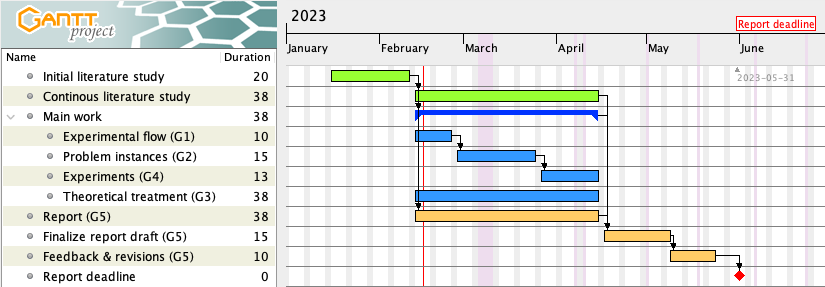
\includegraphics[scale=0.5]{figures/timeline.png} 
	\caption{Time plan for the project.}
	\label{timeplan}
\end{figure}

%\begin{table}[H]
%	\centering
%	\begin{tabular}{c|l}
%		Week(s) & Task \\
%		\hline
%		3-5 & Literature study. \\
%		6-8 & Application \& platform model. [S1-S2] \\
%		9-14 & S3 \\
%		15-17 & Evaluation on hardware. [S4] \\
%		18-20 & Report draft. \\
%		21 & Revisions and final report deadline.
%	\end{tabular}
%    \caption{Preliminary time plan for the project.}
%	\label{timeplan}
%\end{table}

\section{References}
\begin{enumerate}
\item R. Jordão, I. Sander and M. Becker, "Formulation of Design Space Exploration Problems by Composable Design Space Identification," 2021 Design, Automation \& Test in Europe Conference \& Exhibition (DATE), 2021, pp. 1204-1207, doi: 10.23919/DATE51398.2021.9474082.
\item Kathrin Rosvall and Ingo Sander. 2017. Flexible and Tradeoff-Aware Constraint-Based Design Space Exploration for Streaming Applications on Heterogeneous Platforms. ACM Trans. Des. Autom. Electron. Syst. 23, 2, Article 21 (March 2018), 26 pages. \url{https://doi.org/10.1145/3133210}
\item IDeSyDe repository and documentation: \url{https://github.com/forsyde/IDeSyDe/}
\item ForSyDe website: \url{https://forsyde.github.io/}
\end{enumerate}

\end{document}